\chapter{Verwandte Arbeiten}
\todo[inline]{Kapitelname ueberdenken (hab angst vor umlauten in umgebungen), hier auch beschreibung was lambda ueberhaupt ist}
In diesem Kapitel geben wir einen Überblick über bestehende Arbeiten zur Lambda-Architektur und deren Einfluss auf die Entscheidungen, die wir bei der Entwicklung unserer Fallstudie getroffen haben. Zunächst erläutern wir die grundlegende Struktur der Lambda-Architektur, ihre Kernkomponenten und ihre Ziele. Anschließend betrachten wir existierende Implementierungen, die als Inspiration für unser eigenes Fallstudienszenario dienten.

Darauf aufbauend analysieren wir die architektonischen Eigenschaften der Lambda-Architektur sowie ihre bekannten Vor- und Nachteile, um eine Grundlage für die spätere Bewertung unserer Fallstudie zu schaffen. Abschließend vergleichen wir die Lambda-Architektur mit der Kappa-Architektur, einer alternativen Architektur, die in bestimmten Szenarien die Schwächen der Lambda-Architektur umgehen soll.

\section{Überblick über die Lambda-Architektur}
Die Lambda-Architektur wurde von Nathan Marz \cite{warren2015big} als Antwort auf die wachsenden Herausforderungen bei der Verarbeitung großer Datenmengen im Zeitalter von Big Data entwickelt. Sie entstand aus der Erkenntnis, dass herkömmliche Architekturen oft zu komplex, fehleranfällig und schwer skalierbar sind. In vielen Systemen kann bereits ein einziger Datenfehler oder der Ausfall einer Komponente dazu führen, dass das gesamte System inkonsistent wird, Daten verloren gehen oder verfälscht werden und das System nicht mehr zuverlässig arbeitet.

Ein weiteres Problem klassischer Architekturen ist, dass sie Echtzeit- und historische Daten nicht effizient kombinieren können.
Bei Big-Data-Anwendungen muss das System nicht nur jederzeit auf die Daten zugreifen und auf Anfragen reagieren können, sondern auch sicherstellen, dass die gelieferten Informationen stets aktuell sind. Dies würde bedeuten, dass bei jeder einzelnen Anfrage alle gespeicherten Daten vollständig durchsucht und verarbeitet werden müssten, um die aktuellsten Werte zu gewährleisten. Bei wachsenden Datenmengen wird dies jedoch schnell ineffizient und führt zu hohen Latenzzeiten und Systembelastungen.

Um diese Probleme zu lösen, verfolgt die Lambda-Architektur einen Ansatz, der große Datenmengen effizient verarbeitet und gleichzeitig Fehlertoleranz, Skalierbarkeit und Konsistenz gewährleistet.
Hierzu werden Berechnungen nach ihrer Komplexität in Echtzeit- und Batch-Berechnungen unterschieden.
Echtzeit-Berechnungen werden direkt auf eintreffenden Daten ausgeführt und ermöglichen eine aktuellen Überblick.
Hierzu dürfen diese nur wenig Zeit in Anspruch nehmen, weshalb es sich in der Regel um inkrementelle Berechnungen handelt.
Batch-Berechnungen werden periodisch auf der Gesamtheit aller Daten ausgeführt und können eine lange Zeit in Anspruch nehmen.
Diese Berechnungen können beliebig komplex sein, ihre Ergebnisse sind allerdings stets erst verzögert verfügbar.

Das Hauptziel der Lambda-Architektur ist es, 
die aktuellen Daten aus Echtzeit-Berechnungen mit den Ergebnissen der letzten Batch-Berechnungen zu kombinieren,
um Anfragen über historische und aktuelle Daten hinweg zu ermöglichen.
% Hierzu ist eine sorgfältige Einteilung von Berechnungen in Echtzeit-Berechnungen bzw. Batch-Berechnungen notwendig.
Hieraus ergibt sich eine Aufteilung der Architektur in drei Schichten unterteilt (siehe Abbildung 1):

\begin{itemize}
	\item \textbf{Batch Layer:} Speichert alle Rohdaten unverändert und dient als Langzeitarchiv. Dadurch können die Daten wiederholt verarbeitet und für regelmäßige Langzeitanalysen verwendet werden.
	\item \textbf{Speed Layer:} Verarbeitet Datenströme in Echtzeit, um sofortige Ergebnisse zu liefern. Da der Batch-Layer nicht für schnelle Abfragen geeignet ist, übernimmt der Speed-Layer die Aufgabe, aktuelle Daten schnell zur Verfügung zu stellen.
	\item \textbf{Serving Layer:} Verbindet Batch- und Speed-Layer und stellt die Daten für Benutzeranfragen bereit. Kombiniert die Ergebnisse der beiden Schichten und ermöglicht so eine konsistente und effiziente Datenbereitstellung.
\end{itemize}


\begin{figure}[h]
    \centering
    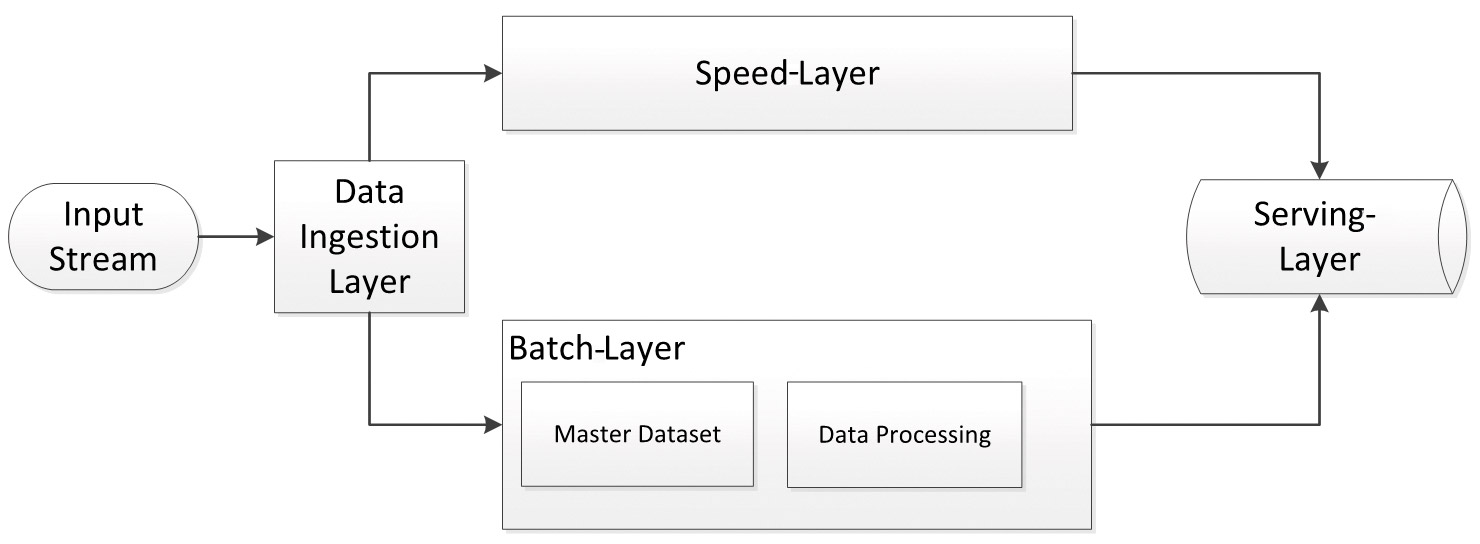
\includegraphics[width=0.8\textwidth]{Graphics/Lambda_Architecture.png}
    \caption{Aufbau der Lambda-Architektur \cite{entwickler_lambda_kappa}.}
    \label{fig:beispielbild}
\end{figure}

Durch diese klare Trennung der Verarbeitungsebenen ermöglicht die Lambda-Architektur ein Gleichgewicht zwischen geringer Latenz und hoher Genauigkeit. Während die Batch Layer eine robuste und fehlertolerante Verarbeitung großer Datenmengen gewährleistet, wäre es zu zeitaufwändig, diese Schicht bei jeder Anfrage vollständig zu durchlaufen, um aktuelle Daten bereitzustellen. Hier kommt der Speed Layer ins Spiel: Er verarbeitet neue Daten in Echtzeit und stellt sie sofort zur Verfügung, um eine schnelle Reaktionszeit zu gewährleisten.

\section{Anwendungsfälle der Lambda-Architektur}
Da traditionelle Systeme wie relationale Datenbanken und klassische Batch-Processing-Systeme zunehmend an ihre Grenzen stoßen, wenn es darum geht, die stetig wachsenden Datenmengen effizient zu verarbeiten, gewinnen Big-Data-Architekturen für moderne Anwendungen immer mehr an Bedeutung. Insbesondere im Zeitalter des Internets, in dem kontinuierlich riesige Datenmengen generiert, übertragen und analysiert werden, hat sich die Lambda-Architektur als leistungsfähige Lösung etabliert \cite{kumar2020lambda,kiran2015lambda,katkar2015study}.

Yuvraj Kumar \cite{kumar2020lambda} beschreibt in seinem Paper eine Vielzahl von modernen Anwendungsfällen der Lambda-Architektur sowie die Technologien, die häufig für deren Implementierung verwendet werden. Große Technologieunternehmen wie Twitter, LinkedIn, Netflix und Amazon nutzen die Lambda-Architektur, um ihre enormen Datenmengen effizient zu analysieren. Vor allem im Bereich der personalisierten Werbung spielt sie eine zentrale Rolle: Historische Kundendaten werden mit aktuellen Nutzerinteraktionen kombiniert, um in Echtzeit maßgeschneiderte Werbung auszuspielen.
Auch im Finanzsektor nutzen Unternehmen die Lambda-Architektur, um historische Transaktionsdaten mit Echtzeitanalysen zu verknüpfen. So können verdächtige Muster identifiziert und Betrugsversuche frühzeitig erkannt werden. Auch im Internet of Things (IoT) findet die Lambda-Architektur breite Anwendung. So wird sie beispielsweise in Smart Cities eingesetzt, um Logistikprozesse zu optimieren oder die Abfallentsorgung effizienter zu gestalten.

Das Paper von Kiran et al. \cite{kiran2015lambda} zeigt, dass insbesondere Smart City Anwendungen stark von der Lambda-Architektur profitieren, da hier große Mengen an Sensordaten kontinuierlich erfasst und analysiert werden müssen. Die Autoren beschreiben eine konkrete Implementierung der Lambda-Architektur zur Verarbeitung und Analyse von Sensordaten in einer Netzwerkumgebung. Hierzu untersuchen Kiran et al. die Verarbeitung von Netzwerk- und Sensordaten aus dem Energy Sciences Network (ESnet). Ziel der Implementierung ist die Erkennung von Anomalien und die Optimierung der Netzwerkauslastung. Die Lamda-Architektur ist für diese Anwendung besonders geeignet, da sie die gleichzeitige Verarbeitung historischer und aktueller Netzdaten ermöglicht. Während im Batch-Layer Langzeitanalysen durchgeführt werden, um wiederkehrende Muster zu identifizieren, kann der Speed-Layer Anomalien in Echtzeit erkennen und darauf reagieren. 

Die in der Literatur beschriebenen Anwendungsfälle, insbesondere die Arbeiten von Kiran et al. \cite{kiran2015lambda} und Kumar \cite{kumar2020lambda}, haben uns geholfen, ein geeignetes Szenario für unsere Fallstudie zu identifizieren. Die Forschung zeigt, dass die Lambda-Architektur besonders häufig in Smart City-Anwendungen eingesetzt wird, da sie die Echtzeitverarbeitung großer Sensordatenströme mit Langzeitanalysen kombiniert.

Darauf aufbauend wollten wir für unsere Fallstudie eine Anwendung im Smart City Kontext wählen, die ebenfalls Echtzeitanalysen mit Langzeitprognosen kombiniert. Dies führte uns schließlich zur Parkhausanalyse. Ähnlich wie in der Arbeit von Kiran et al. \cite{kiran2015lambda} ist es in unserem Szenario sinnvoll, historische Daten zur Vorhersage der Parkhausauslastung mit Echtzeitinformationen über die aktuelle Belegung zu verknüpfen.

\section{Technologien der Lambda-Architektur}
Der vorherige Abschnitt hat gezeigt, dass die Lambda-Architektur eine weit verbreitete Big-Data-Architektur ist, die bereits in einer Vielzahl von Anwendungen implementiert wurde. In der Literatur werden verschiedene Technologien beschrieben, die zur Implementierung der drei Schichten der Lambda-Architektur verwendet werden können.

Ein konkretes Beispiel für die technologische Umsetzung liefert das Paper von Kiran et al. \cite{kiran2015lambda}, das eine Cloud-basierte Implementierung der Lambda-Architektur für die Sensordatenverarbeitung beschreibt. Die Autoren verwenden unterschiedliche Technologien für den Batch Layer, den Speed Layer und den Serving Layer.

Für den Batch Layer verwenden Kiran et al. \cite{kiran2015lambda} das Apache Hadoop Distributed File System (HDFS). HDFS ist eine der am häufigsten verwendeten Technologien für die Lambda-Architektur, da es ein skalierbares, fehlertolerantes und verteiltes Dateisystem darstellt, das speziell für die Speicherung großer Datenmengen entwickelt wurde \cite{ganelin2016spark}.
Aufgrund seiner Architektur ist HDFS jedoch relativ langsam bei Lese- und Schreibzugriffen, weshalb es hauptsächlich für Batch-Processing-Aufgaben verwendet wird. In der Implementierung von Kiran et al. wird HDFS verwendet, um historische Rohsensordaten von Netzwerkroutern unverändert zu archivieren. Da Lesezugriffe auf HDFS relativ langsam sind, können periodische Batch-Analysen sehr zeitaufwändig sein.

Für die Speed Layer verwenden Kiran et al. \cite{kiran2015lambda} Apache Spark Streaming. Apache Spark ist eine vielseitige Technologie, die sowohl für Batch Processing als auch für Stream Processing eingesetzt werden kann. Spark Streaming ist eine Erweiterung von Apache Spark und ermöglicht die Verarbeitung von Datenströmen in Echtzeit, indem eingehende Daten kontinuierlich analysiert und aggregiert werden.
Der Vorteil von Spark Streaming gegenüber klassischen Batch-Technologien ist, dass es Echtzeitdatenverarbeitung mit geringer Latenz ermöglicht, ohne dass die Daten vorher vollständig gespeichert werden müssen.

Für den Serving Layer verwenden Kiran et al. \cite{kiran2015lambda} Amazon S3, um die Sensordaten aus dem Batch Layer zu aggregieren und für historische und Echtzeit-Abfragen bereitzustellen. Die Wahl von Amazon S3 basiert darauf, dass die Autoren eine Cloud-basierte Implementierung der Lambda-Architektur entwickelt haben, die auf skalierbare Speicherdienste angewiesen ist.

Im Gegensatz dazu planen wir in unserer Fallstudie eine lokale Implementierung der Lambda-Architektur, weshalb alternative Technologien für die Speicherung und Aggregation im Serving Layer in Betracht gezogen werden müssen.

In der Literatur werden zahlreiche weitere Technologien beschrieben, die für die verschiedenen Schichten der Lambda-Architektur eingesetzt werden können. Besonders hervorzuheben ist die Arbeit von Kumar \cite{kumar2020lambda}, der mehrere alternative Technologien diskutiert, die auch für unsere Fallstudie vielversprechend sind.

Laut Kumar \cite{kumar2020lambda} ist Apache Kafka eine der am häufigsten verwendeten Technologien für die Lambda-Architektur. Kafka ist ein verteiltes Publish-Subscribe-Messaging-System, das für Echtzeit-Datenströme optimiert ist \cite{kreps2011kafka}. Es ermöglicht das Publizieren neuer Daten in Echtzeit in eine Queue. Von dort aus können die Daten sowohl an den Batch-Layer zur langfristigen Speicherung als auch an den Speed-Layer zur sofortigen Verarbeitung weitergeleitet werden. Damit ist sichergestellt, dass Echtzeit- und Langzeitverarbeitung parallel erfolgen können.

Eine weitere Technologie, die laut Kumar \cite{kumar2020lambda} häufig in der Lambda-Architektur eingesetzt wird, ist Apache Cassandra. Cassandra ist eine hochskalierbare NoSQL-Datenbank, die sich besonders für den Serving Layer eignet \cite{warren2015big}. Im Serving Layer werden Echtzeitabfragen aus dem Speed Layer und aggregierte Batch Views aus dem Batch Layer zusammengeführt und gespeichert. Cassandra zeichnet sich durch schnelle Lese- und Schreibzugriffe aus, was für die kontinuierliche Aktualisierung der Daten im Serving Layer wichtig ist.

\section{Eigenschaften der Lambda-Architektur}
Nachdem wir uns in den vorherigen Abschnitten mit verschiedenen Anwendungsfällen und Technologien der Lambda-Architektur beschäftigt haben, wollen wir nun die zentralen Eigenschaften dieser Architektur näher analysieren. Basierend auf den betrachteten Anwendungsfällen identifizieren wir die wesentlichen Stärken und Schwächen der Lambda-Architektur. Diese identifizierten Eigenschaften wollen wir später als Richtlinien für die Implementierung und Evaluierung unserer Fallstudie nutzen.

\subsection{Vorteile der Lambda-Architektur}
Die Lambda-Architektur zeichnet sich durch eine klare Trennung der Datenverarbeitung in drei Schichten aus. Diese Struktur ermöglicht es, jede Schicht unabhängig voneinander zu optimieren und weiterzuentwickeln. Wie Marz \cite{warren2015big} beschreibt, sind die einzelnen Verarbeitungsebenen nur gering voneinander abhängig, so dass sie mit unterschiedlichen Technologien realisiert werden können. Dadurch kann jede Schicht flexibel ausgetauscht oder skaliert werden, ohne dass die gesamte Architektur überarbeitet werden muss. Diese Skalierbarkeit macht die Lambda-Architektur besonders geeignet für Big-Data-Anwendungen, da sie flexibel an steigende Datenmengen angepasst werden kann.

Ein weiteres zentrales Merkmal der Lambda-Architektur ist die Fehlertoleranz durch die Verwendung von Immutable Data \cite{warren2015big}. Da die Rohdaten unverändert in der Batch Layer gespeichert werden, bleiben sie jederzeit abrufbar und können erneut verarbeitet werden, ohne dass das System inkonsistent wird. Marz \cite{warren2015big} betont, dass dieser Ansatz Datenverluste nahezu ausschließt, da Daten nicht gelöscht oder überschrieben, sondern nur ergänzt werden. Tritt ein Fehler in der Verarbeitung oder in den Daten selbst auf, kann dieser durch eine erneute Verarbeitung der unveränderten Rohdaten behoben werden. Dies ist insbesondere in Anwendungen mit hohen Anforderungen an die Datenintegrität von Vorteil. Die Arbeit von Kiran et al. \cite{kiran2015lambda} zur Netzwerkanalyse im ESnet zeigt, dass diese Eigenschaft es ermöglicht, Sensordaten langfristig zu speichern und Fehler in der Netzwerkanalyse durch Nachberechnungen zu korrigieren.

\subsection{Nachteile der Lambda-Architektur}
Obwohl die Lambda-Architektur viele Vorteile bietet, bringt sie auch Nachteile mit sich. 

Die Trennung der Verarbeitungsebenen führt zu einem erhöhten Entwicklungs- und Wartungsaufwand. 
Die von Marz \cite{warren2015big} beschriebene geringe Abhängigkeit zwischen den Schichten bietet zwar Flexibilität, 
allerdings ergibt sich auch ein geringes Potenzial für gemeinsame Implementierungen beziehungsweise die Wiederverwendung von Komponenten.
Dies trifft umso mehr zu, wenn die Schichten unterschiedliche Technologien einsetzen.

Kumar \cite{kumar2020lambda} beschreibt insbesondere die hohe Komplexität der Kombination von Speed Layer und Batch Layer im Serving Layer. Da für beide Verarbeitungsebenen separate Pipelines entwickelt werden müssen, ist es notwendig, die Ergebnisse beider Ebenen in der Serving Layer zu integrieren. Diese Integration kann fehleranfällig sein und erfordert eine sorgfältige Synchronisation der Daten, um konsistente Abfragen zu gewährleisten. Während die Lambda-Architektur auf konzeptioneller Ebene einfach zu verstehen ist, stellt die technische Umsetzung eine Herausforderung dar. Die verschiedenen Schichten werden mit unterschiedlichen Open-Source-Technologien realisiert, die miteinander kommunizieren müssen \cite{katkar2015study}.

Ein weiteres Problem der Lambda-Architektur ist der hohe Speicherbedarf durch die doppelte Datenhaltung. Da sowohl die Speed Layer als auch die Batch Layer Daten speichern, werden viele Daten redundant gespeichert, um eine konsistente Verarbeitung in beiden Schichten zu gewährleisten. Während der Batch-Layer alle Rohdaten langfristig speichert, verwendet der Speed-Layer einen separaten Speicher für die Echtzeitverarbeitung. Dies führt insbesondere bei Anwendungen mit großen Datenmengen zu einem erhöhten Speicherbedarf \cite{kumar2020lambda}.